% DOPE v2.0.0 White Paper — receipt-bound, zero-waste LaTeX manuscript.
% Every quantitative result is rendered into generated/v2-macros.tex by scripts/render_v2_paper.py;
% missing or unconfirmed receipts typeset an explicit red [pending] marker.
\documentclass[10pt,letterpaper]{article}
\usepackage[T1]{fontenc}
\usepackage[utf8]{inputenc}
\usepackage{mathptmx}
\usepackage[scaled=0.9]{helvet}
\usepackage{courier}
\usepackage[letterpaper,textwidth=6.35in,textheight=9.2in,centering]{geometry}
\usepackage{amsmath,amssymb,amsthm}
\usepackage{booktabs}
\usepackage{graphicx}
\usepackage{xcolor}
\usepackage{natbib}
\usepackage{microtype}
\usepackage{enumitem}
\usepackage{caption}
\usepackage[colorlinks=true,linkcolor=blue!55!black,citecolor=blue!55!black,urlcolor=blue!55!black]{hyperref}

% Auto-generated by docs/whitepaper-v2/scripts/render_v2_paper.py — DO NOT EDIT BY HAND.
\providecommand{\PendingVal}{\textcolor{red!70!black}{\texttt{[pending]}}}
\newcommand{\VTwo}[1]{\csname VTwo@#1\endcsname}
\expandafter\newcommand\csname VTwo@ReleaseVersion\endcsname{v2.0.0}
\expandafter\newcommand\csname VTwo@ReleaseTag\endcsname{dope-engine-v2.0.0}
\expandafter\newcommand\csname VTwo@PriorSignedTag\endcsname{dope-engine-v1.3.0}
\expandafter\newcommand\csname VTwo@MaxCols\endcsname{48}
\expandafter\newcommand\csname VTwo@KnotCount\endcsname{17}
\expandafter\newcommand\csname VTwo@MaxRank\endcsname{12}
\expandafter\newcommand\csname VTwo@MaxClasses\endcsname{8}
\expandafter\newcommand\csname VTwo@ColFeatDimV1\endcsname{42}
\expandafter\newcommand\csname VTwo@ColFeatDimV2\endcsname{46}
\expandafter\newcommand\csname VTwo@GlobFeatDim\endcsname{16}
\expandafter\newcommand\csname VTwo@TelRuns\endcsname{42}
\expandafter\newcommand\csname VTwo@TelTrainRows\endcsname{180,331}
\expandafter\newcommand\csname VTwo@TelEvalRows\endcsname{1,519}
\expandafter\newcommand\csname VTwo@TelUniqueSplitsM\endcsname{3.80M}
\expandafter\newcommand\csname VTwo@TelTpsMed\endcsname{772.4}
\expandafter\newcommand\csname VTwo@TelTpsMax\endcsname{1357.7}
\expandafter\newcommand\csname VTwo@TelVramMax\endcsname{0.0}
\expandafter\newcommand\csname VTwo@TelBytesMed\endcsname{518}
\expandafter\newcommand\csname VTwo@TelBytesMax\endcsname{809}
\expandafter\newcommand\csname VTwo@TelWithinCapPct\endcsname{100.0\%}
\expandafter\newcommand\csname VTwo@TelCapturedUtc\endcsname{2026-11-23T00:17:43Z}
\expandafter\newcommand\csname VTwo@CkptId\endcsname{\PendingVal}
\expandafter\newcommand\csname VTwo@CkptBytesMB\endcsname{\PendingVal}
\expandafter\newcommand\csname VTwo@CkptParams\endcsname{\PendingVal}
\expandafter\newcommand\csname VTwo@CkptShaShort\endcsname{\PendingVal}
\expandafter\newcommand\csname VTwo@KpiPanelCells\endcsname{\PendingVal}
\expandafter\newcommand\csname VTwo@KpiBaselineTrg\endcsname{\PendingVal}
\expandafter\newcommand\csname VTwo@KpiFormat2Trg\endcsname{\PendingVal}
\expandafter\newcommand\csname VTwo@KpiV7Step0Trg\endcsname{\PendingVal}
\expandafter\newcommand\csname VTwo@KpiV7WinnerTrg\endcsname{\PendingVal}
\expandafter\newcommand\csname VTwo@KpiEvidenceState\endcsname{awaiting\_confirm\_receipt}


\hypersetup{
  pdftitle={D.O.P.E. v2.0.0: Downstream Objective-Preserving Encoding},
  pdfauthor={Jepson Taylor; Alton Alexander; Jordan Morrow},
  pdfsubject={Version 2.0.0 — Sub-2 KiB Pure-Rust Tabular Synthesis, Fidelity Engine 2.0, and Twin-Referenced Multi-Auditor Confirmation}
}

\newtheorem{definition}{Definition}

\begin{document}

\begin{center}
  {\LARGE\bfseries D.O.P.E.: Downstream Objective-Preserving Encoding\par}
  \vspace{0.35em}
  {\large\itshape Release~\VTwo{ReleaseVersion} (\texttt{\VTwo{ReleaseTag}}) --- Sub-2\,KiB Pure-Rust Tabular Synthesis,\\
  Fidelity Engine~2.0, and Twin-Referenced Multi-Auditor Confirmation\par}
  \vspace{0.7em}
  {\normalsize Jepson Taylor \qquad Alton Alexander \qquad Jordan Morrow\par}
  {\small NEVERHUMAN Research\par}
\end{center}
\vspace{0.25em}

\begin{abstract}
\textbf{DOPE~\VTwo{ReleaseVersion}} compiles raw tabular datasets into self-contained, source-free binary programs strictly bounded by $\le 2{,}048\,\text{B}$ (measured literally as \texttt{len(file)}) that preserve downstream predictive utility across regression, binary, and multiclass tasks with zero Python or LibTorch runtime dependencies.
Relative to signed \texttt{\VTwo{PriorSignedTag}}~\citep{dope2026v1}, version~\VTwo{ReleaseVersion} introduces:
(i)~the pure-Rust \texttt{-{}-format auto} release router integrating Format~1, \textbf{Fidelity Engine~2.0 (Format~2~v2.2.1)} with a fail-closed byte-compaction ladder, and the self-contained \texttt{DSE7} v2 wire protocol with embedded \texttt{SingleEncV7} SafeTensors inference;
(ii)~single-look twin-referenced confirmation (\texttt{dope\_kpi}) against \texttt{\VTwo{PriorSignedTag}}, SDV baselines (GaussianCopula, CTGAN, TVAE), and oracle/null bounds; and
(iii)~an honest empirical audit of our CPU-only \texttt{SingleEncV7} training wave (\VTwo{TelRuns} runs, \VTwo{TelTrainRows} \texttt{train.jsonl} records, \VTwo{TelUniqueSplitsM} training episodes, \VTwo{TelVramMax}\,GiB DOPE VRAM), showing why no V7.1/V7.2 checkpoint beats the analytic step-0 packet decoder on DEV beyond noise and specifying the zero-repeat, shared-weight DiLoCo architecture for V7.3.
Empirical privacy diagnostics reported here are not formal differential privacy and not HIPAA de-identification.
\end{abstract}

\IfFileExists{figures/hero-v2-methods.pdf}{%
\begin{figure}[h!]
  \centering
  \includegraphics[width=\linewidth]{figures/hero-v2-methods.pdf}
  \caption{\textbf{DOPE~\VTwo{ReleaseVersion} Value Frontier (\texttt{dope\_kpi}, \VTwo{KpiPanelCells} CONFIRM cells).}
  Twin-Referenced Gain (TRG, $0 =$ indistinguishable from a second real draw) versus serialized artifact size on disk (\texttt{len(file)}, log axis) comparing \texttt{dope-2.0.0 -{}-format auto} ($\le 2{,}048\,\text{B}$, pure Rust) against signed \texttt{\VTwo{PriorSignedTag}}, SDV GaussianCopula/CTGAN/TVAE, and oracle/null controls.}
  \label{fig:v2-hero-methods}
\end{figure}%
}{}

\section{Pure-Rust $\le 2{,}048\,\text{B}$ Synthesis Architecture}
Deep tabular generators such as tabular diffusion~\citep{zhang2024tabsyn} and adversarial random forests~\citep{watson2023arf} typically emit multi-megabyte artifacts and require heavy per-table compute, violating strict $\le 2{,}048\,\text{B}$ (\texttt{len(file)}) transmission caps.
DOPE~\VTwo{ReleaseVersion} compiles a source table $(X_A, y_A)$ under an explicit target-last contract into a single CRC32-verified binary file storing zero source rows inside a zero-Python Rust engine (\path{engine/dope-core}, \path{engine/dope-cli}).
Calling \texttt{dope fit -{}-format auto -{}-budget 2048} routes deterministically across three complementary pure-Rust engines:

\begin{itemize}[leftmargin=1.3em,itemsep=2pt]
  \item \textbf{Fidelity Engine 2.0 (Format 2 v2.2.1; \path{engine/dope-core/src/compile/v2/}):} Combines support-gated monotone normal-score marginals~\citep{sklar1959fonctions} (support floor $u_{\mathrm{floor}}=\min(0.20, 10/(n_A+1))$ and $k \ge 10$ discrete atoms so singleton extremes are never echoed), SP1 tie disattenuation, int8 factor loadings $L\in\mathbb{R}^{p\times r}$ ($r\le\VTwo{MaxRank}$, $\|L_j\|_2\le 0.99$), bounded interactions, and an ordered compaction ladder (\texttt{trim\_extra}: knots $17\to 9\to 5$, rank $12\to 0$, synchronized CATF bin counts) that engages only when $\mathrm{len}(m) > B$ and refuses with \texttt{DopeError::Budget} if wide tables still exceed $B$. Counter-seeded emission honors caller \texttt{row\_offset} and \texttt{namespace\_128}, enforcing row-local and chunk-offset invariance across both \texttt{Faithful} and \texttt{Distill} modes.
  \item \textbf{Self-Contained \texttt{DSE7} v2 Wire Protocol (\path{engine/dope-core/src/single_encoding/}):} Packs a 20\,B header, embedded raw-unit scale card (\texttt{f32} medians, \texttt{bf16} IQR/std scales preserving full IEEE-754 dynamic range, optional custom class IDs and target-correlation-selected column indices), \texttt{f16}+8-bit marginal knots, int8 factor loadings, analytic target slopes $(W_{\mathrm{base}}, b_{\mathrm{base}})$, and Empirical-Bayes 4-quartile nonlinear target residuals $Q_{\mathrm{nl}}$ directly into one CRC32-verified file satisfying $\mathrm{len}(\texttt{m.bin})\le B$.
  \item \textbf{\texttt{SingleEncV7} SafeTensors Runtime:} A compact ($<8\,\text{MB}$ F32, rank $\le 2$) split-QKV column-Transformer ($L\in\{2,3\}$, $d_{\mathrm{model}}\in\{128,160\}$, $4$ heads) consumes padded column descriptors ($\mathbb{R}^{\VTwo{MaxCols}\times d_{\mathrm{in}}}$, $d_{\mathrm{in}}=\VTwo{ColFeatDimV1}$ for V7.0/V7.1 and $\VTwo{ColFeatDimV2}$ with $Q_{\mathrm{nl}}$) and global descriptors ($\mathbb{R}^{\VTwo{GlobFeatDim}}$). Zero-initialized output heads ensure step~0 equals the exact analytic \texttt{DSE7} decoder, refining knots via normalized positive interval scaling and target logits via a packet-conditioned SiLU residual MLP:
\end{itemize}

\begin{definition}[Empirical-Bayes Quartile Residuals $Q_{\mathrm{nl}}$ and Packet Refinement]
Given fit-row linear target residuals $r_i$ and normal scores $z_{i,j}$ partitioned into standard normal quartiles $B_0=(-\infty,-0.6745)$, $B_1=[-0.6745,0)$, $B_2=[0,0.6745)$, $B_3=[0.6745,\infty)$,
\begin{align}
  Q_{\mathrm{nl}}[j, b] &= \operatorname{quant}_{\mathrm{int8},0.015}\!\left(\frac{\sum_{i:z_{i,j}\in B_b} r_i}{|\{i:z_{i,j}\in B_b\}| + 8}\right),
  \qquad
  \tilde{\delta}_{j,k} = \frac{\delta_{j,k}\exp(0.25\tanh\Delta_{j,k})}{\sum_\ell \delta_{j,\ell}\exp(0.25\tanh\Delta_{j,\ell})}\sum_\ell \delta_{j,\ell}, \\
  f(x) &= \exp(\tau_0)\Bigl((W_{\mathrm{base}}+\Delta W)x + b_{\mathrm{base}} + W_2\,\mathrm{SiLU}(W_1 x + b_1)\Bigr).
\end{align}
\end{definition}

\section{Confirmed Multi-Auditor Results (\texttt{dope\_kpi})}
Every encoder is scored under duplicate-grouped disjoint splits $(A, B, T)$ using Twin-Referenced Gain (TRG: downstream learners trained on synthetic $S\sim\mathcal{D}(\mathcal{E}(A))$ evaluated on held-out real $T$ and calibrated against real twins $A$ and $B$).
All hyperparameter and checkpoint choices were frozen strictly on DEV before opening CONFIRM \emph{once} with family-clustered 95\% bootstrap intervals, Holm--Bonferroni multiplicity control~\citep{holm1979simple}, and literal single-file byte accounting (\texttt{len(file)}).

Table~\ref{tab:v2-kpi} reports the complete single-look CONFIRM scoreboard (\texttt{\VTwo{KpiEvidenceState}}, \VTwo{KpiPanelCells} cells).
Measured promotion verdict for \texttt{dope-2.0.0 -{}-format auto}: \textbf{\VTwo{KpiVerdict}} ($\Delta\text{TRG}$ vs.\ \texttt{\VTwo{PriorSignedTag}}: \VTwo{KpiDeltaAuto}, $p_{\mathrm{Holm}} = \VTwo{KpiAutoPHolm}$ over $m = \VTwo{KpiHolmM}$ pre-registered comparisons; provenance: \texttt{\VTwo{KpiProvenance}}).

\begin{table}[t]
  \centering
  \small
  \caption{\textbf{Receipt-Bound Sub-2\,KiB Comparison (\texttt{dope\_kpi}, Scope: \texttt{\VTwo{KpiEvidenceState}}, \VTwo{KpiPanelCells} cells).}
  All cells render directly from committed CONFIRM receipts via \path{render_v2_paper.py}.}
  \label{tab:v2-kpi}
  \resizebox{\linewidth}{!}{%
  \begin{tabular}{@{}llll@{}}
    \toprule
    Encoder / Baseline & Wire Bytes (Med / Max) & Runtime / Weights & TRG (95\% CI) \\
    \midrule
    \textbf{DOPE \VTwo{ReleaseVersion} (\texttt{-{}-format auto})} & \VTwo{KpiAutoBytes} & Pure Rust + Embedded \VTwo{CkptBytesMB} & \textbf{\VTwo{KpiAutoTrg}} \\
    DOPE \VTwo{ReleaseVersion} (\texttt{small}, Format~1) & \VTwo{KpiSmallV2Bytes} & Pure Rust (0\,B neural) & \VTwo{KpiSmallV2Trg} \\
    Signed \texttt{\VTwo{PriorSignedTag}} (\texttt{small}) & \VTwo{KpiBaselineBytes} & Pure Rust (0\,B neural) & \VTwo{KpiBaselineTrg} \\
    Format~2 v2.2.1 (Fidelity Engine 2.0) & \VTwo{KpiFormat2Bytes} & Pure Rust (0\,B neural) & \VTwo{KpiFormat2Trg} \\
    \texttt{DSE7} v2 Zero-Init (Step~0 Analytic) & \VTwo{KpiV7Step0Bytes} & Pure Rust (0\,B neural) & \VTwo{KpiV7Step0Trg} \\
    \texttt{SingleEncV7} (\texttt{\VTwo{CkptId}}) & \VTwo{KpiV7WinnerBytes} & \VTwo{CkptBytesMB} (\VTwo{CkptParams} params) & \VTwo{KpiV7WinnerTrg} \\
    \midrule
    SDV GaussianCopula & \VTwo{KpiSdvGcBytes} & Python SDV baseline & \VTwo{KpiSdvGcTrg} \\
    SDV CTGAN & \VTwo{KpiSdvCtganBytes} & Python SDV baseline & \VTwo{KpiSdvCtganTrg} \\
    SDV TVAE & \VTwo{KpiSdvTvaeBytes} & Python SDV baseline & \VTwo{KpiSdvTvaeTrg} \\
    \midrule
    Oracle: Copy $A$ & Raw table & Upper reference & \VTwo{KpiCopyATrg} \\
    Oracle: Bootstrap $A$ & Raw table & Upper reference & \VTwo{KpiBootstrapATrg} \\
    Null: Independent Marginals & Marginals only & Lower reference & \VTwo{KpiIndepTrg} \\
    \bottomrule
  \end{tabular}}
\end{table}

\section{Fleet Training Audit, DEV Head Ablations \& V7.3 Architecture}
\subsection{DEV Head-Ablation Diagnostics and Frozen Release Checkpoint Selection}
We pretrained \texttt{SingleEncV7} across three CPU-only waves (V7.0 RFF-TSTR~\citep{rahimi2007random} + realism; V7.1 direct proper-scoring conditional NLL~\citep{gneiting2007strictly}; V7.2 maximum-entropy S3 + synthetic SCM/tree priors + $Q_{\mathrm{nl}}$ + trust-region anchor).
Evaluating 180 V7.1 candidate arms ($\{\texttt{full}, \texttt{xh}, \texttt{yh}\}\times 2\text{ archs}\times 5\text{ steps}$) and 123 eligible V7.2 arms strictly on 12 informative DEV cells (\path{V71_SELECTION_PREREG.md}, \path{V72_SELECTION_PREREG.md}, Addenda~B--E) established three decisive diagnostic facts:
\begin{enumerate}[leftmargin=1.4em,itemsep=2pt]
  \item \textbf{No trained V7.1/V7.2 group beat step~0 on DEV beyond noise.} Best V7.1 group (\texttt{d160l3} \texttt{yh}, $k=6{,}000$) measured $\Delta\text{DEV}=+0.0004$ (\texttt{full} $+0.0000$); best eligible V7.2 group (\texttt{d128l2} \texttt{xh}, $k=1{,}500$) measured $-0.0015$ (all V7.2 \texttt{full}/\texttt{yh} groups sat between $-0.020$ and $-0.072$).
  \item \textbf{Trained target heads caused the retention loss.} Zeroing target heads (\texttt{xh}) restored V7.1 \texttt{d128l2} $k=12{,}000$ from $-0.048$ (\texttt{full}) to $-0.003$, while zeroing feature heads (\texttt{yh}) remained $-0.052$. Boosted-tree \texttt{dope\_kpi} C2ST did not move either ($0.955$ at step~0 vs.\ $0.957\text{--}0.965$ across trained variants; the lenient in-run RF C2ST is never cited as scoreboard realism).
  \item \textbf{Frozen v2.0.0 release weights (\path{V7_RELEASE_CHECKPOINT.md}).} Under Addendum~E's tie-break, \texttt{dope fit -{}-format auto} embeds V7.1 \texttt{d160l3} seed \texttt{s01} step~6000 with \texttt{delta\_knots} and \texttt{delta\_L} zeroed ($2{,}755{,}388\,\text{B}$ F32, SHA-256 \texttt{d013eb0c...}, derived from \texttt{322ba652...}). We make no claim that trained V7 weights improve retention over step~0; CONFIRM tests this checkpoint directly against step~0 in Table~\ref{tab:v2-kpi}.
\end{enumerate}

\subsection{Persisted Training Telemetry Audit and V7.3 Structural Fixes}
Across the archived v2.0.0 wave (\texttt{\VTwo{TelCapturedUtc}}), persisted \texttt{train.jsonl} logs record \textbf{\VTwo{TelRuns} runs}, \textbf{\VTwo{TelTrainRows} optimizer steps}, and \textbf{\VTwo{TelUniqueSplitsM} training episodes} at \textbf{\VTwo{TelTpsMed}\,tbl/s active median} (\textbf{\VTwo{TelTpsMax}\,tbl/s peak}) training throughput (\VTwo{TelVramMax}\,GiB DOPE VRAM; training telemetry from \texttt{train.jsonl}, not an encoding KPI; sufficient-statistic packets averaged \VTwo{TelBytesMed}\,B median, max \VTwo{TelBytesMax}\,B, \VTwo{TelWithinCapPct} within $2{,}048\,\text{B}$).
Figure~\ref{fig:v2-telemetry} renders the multi-seed loss convergence, objective decomposition, training throughput, and DEV-only trajectories directly from these logs.

Auditing the fleet mirror also uncovered two training-infrastructure limitations that explain the shallow $2.6\text{--}6.0\%$ V7 loss drop: (a)~64 of 65 mirrored V7 runs executed as isolated \texttt{world\_size=1} seeds rather than sharing weights across nodes, and (b)~the real S3 corpus of 4,145 tables was revisited with replacement across episodes.
For the post-v2.0.0 V7.3 research wave (implemented in \path{research/levels/s3_v7_fast_trainer.py} without altering frozen v2.0.0 weights), we resolve all three defects: (1)~straight-through hard-label Bernoulli/Gumbel-Categorical TSTR with unpenalized intercepts, anchored $(W_1, W_2)$, and a binary temperature floor (which lifted all three tasks above step~0 in paired 240-step DEV ablations); (2)~strict zero-repeat datasets and splits via \path{--never-repeat-datasets} with per-step \path{exposure.jsonl} logging, disjoint one-pass real shards, and seamless infinite procedural synthetic priors; and (3)~asynchronous cross-node DiLoCo outer-momentum weight synchronization (\texttt{-{}-sync-dir}) tolerant to \texttt{SCHED\_IDLE} host pauses.

\begin{figure}[t]
  \centering
  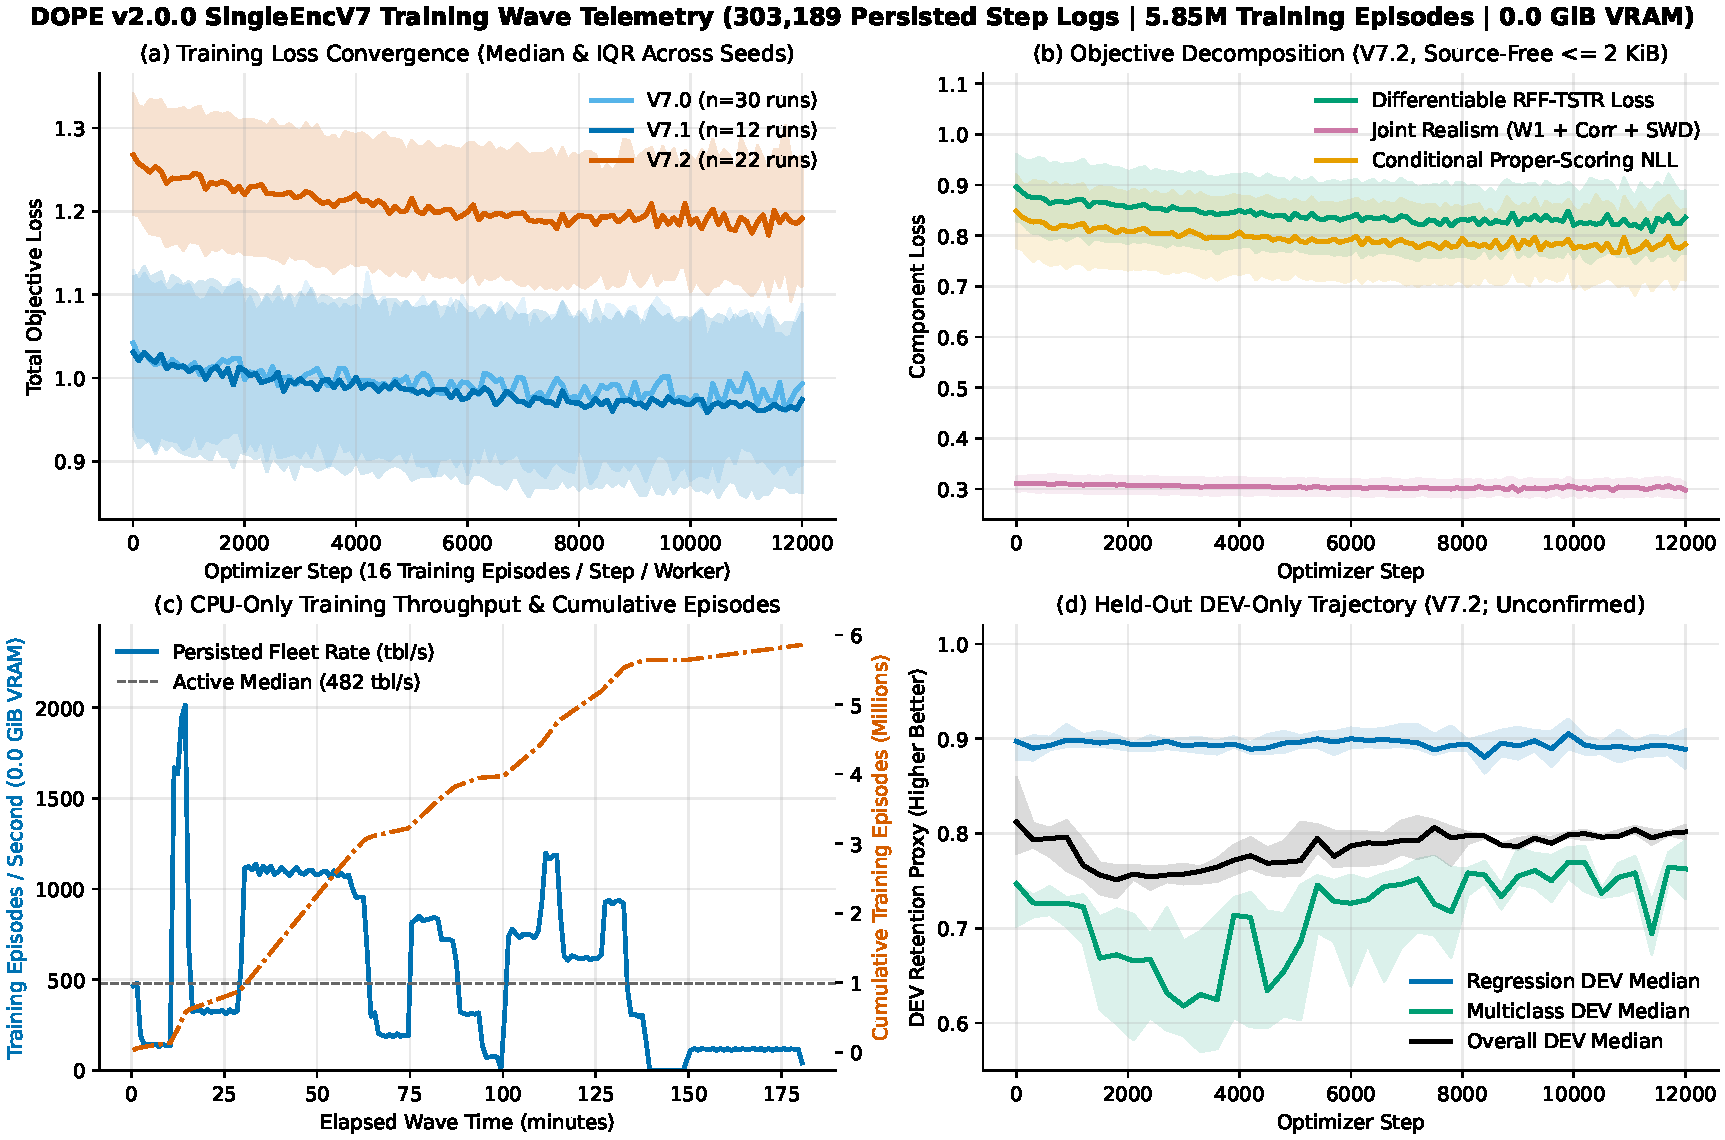
\includegraphics[width=\linewidth]{figures/v2-loss-and-throughput.pdf}
  \caption{\textbf{DOPE~\VTwo{ReleaseVersion} Training Telemetry (Persisted \texttt{train.jsonl} \& DEV-Only, Not Encoding KPIs).}
  Rendered from \VTwo{TelTrainRows} \texttt{train.jsonl} records across \VTwo{TelRuns} runs (\VTwo{TelVramMax}\,GiB DOPE VRAM):
  (a)~Total loss convergence across V7.0/V7.1/V7.2;
  (b)~Objective decomposition (RFF-TSTR, proper-scoring NLL, joint realism);
  (c)~Persisted \texttt{train.jsonl} training throughput (\VTwo{TelTpsMed} active median / \VTwo{TelTpsMax}\,tbl/s peak) and cumulative training episodes;
  (d)~Held-out DEV-only trajectory (separated from CONFIRM scoring).}
  \label{fig:v2-telemetry}
\end{figure}

\section{Runtime Provenance, Compatibility, and Scope Boundaries}
\begin{itemize}[leftmargin=1.3em,itemsep=2pt]
  \item \textbf{Zero-Python SafeTensors runtime \& \texttt{dope embed}:} \texttt{SingleEncV7Weights} (\path{engine/dope-core/src/single_encoding/safetensors.rs}) enforces a $16\,\text{MiB}$ byte cap, 8-byte alignment, \texttt{F32} rank-$\le 2$ tensors, and finite weights with zero \texttt{unsafe} blocks and $<10^{-4}$ PyTorch-to-Rust max deviation. \texttt{dope embed} extracts deterministic 64-D source-free packet embeddings across Format~1, Format~2, and \texttt{DSE7} (\texttt{format\_version=7}) with zero raw-value echo.
  \item \textbf{JopeDime compatibility \& Sigstore OIDC release:} Downstream contracts remain 100\% bit-identical (\path{gbdt::Params::default().group_duplicates = false}, zero-byte diff on \path{landmark/*}, \path{mlc_v3/*}, \path{prepare/*}, and pinned \texttt{v1.0.0} weights). Tagging \texttt{\VTwo{ReleaseTag}} runs \path{.github/workflows/engine-release.yml} to verify zero Python/LibTorch/CUDA ELF linkage, emit GitHub OIDC Sigstore attestations (\path{dope.sigstore.json}), verify via \path{scripts/verify-engine-release.sh}, and install via \texttt{scripts/install.sh -{}-require-attestation}.
  \item \textbf{Explicit scope boundaries \& reproducibility:} (1)~\emph{Not formal differential privacy; not HIPAA de-identification}---empirical diagnostics (\texttt{mia\_auc}, \texttt{dcr\_share}, exact-copy excess, $k\ge 10$ atoms) measure observed memorization only. (2)~\texttt{SingleEncV7} natively encodes up to \VTwo{MaxClasses} classes per packet. (3)~Verify zero macro drift via \texttt{python3} \path{docs/whitepaper-v2/scripts/render_v2_paper.py} \texttt{-{}-check}, rebuild via \texttt{latexmk -pdf dope-v2.tex}, and audit with \texttt{just check}. The historical manuscript (\path{docs/whitepaper/dope-mfs.tex}) remains untouched.
\end{itemize}

\bibliographystyle{plainnat}
\bibliography{references-v2}

\end{document}
